This layer will consist of an Amp and Speaker combination. The amplifier will take the sound signals and increase them granted there is no distortion to output a clean and powerful sound from the speakers.

\subsection{Audio Amplifier}
The Amplifier increases the amplitude of electrical signals for sound reproduction. The amplifier consists of two main parts. The Pre-Amplifier and the Amplifier. These 2 components will work together to deliver a controlled sound signal for a speaker to play.

\begin{figure}[h!]
	\centering
 	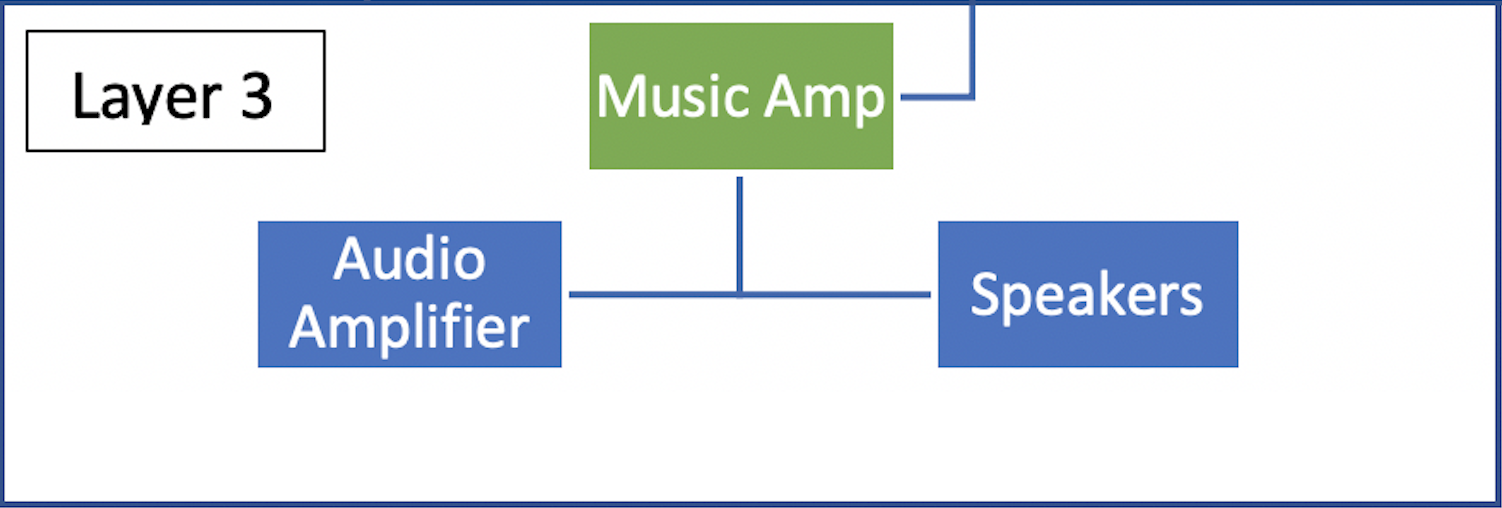
\includegraphics[width=0.60\textwidth]{images/subsystem3}
 \caption{Music amplification subsystem - audio amplifier}
\end{figure}

\subsubsection{Assumptions}
Amplifier increases amplitude of electrical signals for sound reproduction. This is done by switching the signals from AC to DC which can be passed onto transistors for further processing.

\subsubsection{Responsibilities}
The amplifier is responsible for adjusting the intensity of the sound signals to be registered properly by a speaker. The pre-amp is able to provide the current gain required for the speaker, and the amplifier adjusts the intensity even more which is why the amplifier is so important. The pre-amp is also responsible for bringing signals to the level line.

The audio amplifier allows for volume control. This allows the pre-amp to deliver controlled inputs to the Amp. The amp then takes the signals and amplifies it power wise to deliver a more clear, vibrant, deep, and powerful sound to the speaker. With high energy consumption, the amplifier also releases excess heat which is usually handled with heat sinks and airways for passive cooling.

\subsubsection{Subsystem Interfaces}
\begin {table}[H]
\caption {Audio amplifier interfaces} 
\begin{center}
    \begin{tabular}{ | p{1cm} | p{6cm} | p{3cm} | p{3cm} |}
    \hline
    ID & Description & Inputs & Outputs \\ \hline
    \#5 & Pre-Amplifier & \pbox{3cm}{Sound signals from device} & \pbox{3cm}{Signals to Amplifier}  \\ \hline
    \#6 & Amplifier & \pbox{3cm}{Signals from Pre-Amplifier} & \pbox{3cm}{Amplified Signals to Speaker}  \\ \hline
    \end{tabular}
\end{center}
\end{table}

\subsection{Speakers}
The speakers are one of the last, most straightforward systems in the backpack. There will be three sets of speakers for different frequencies: lows, mids, and highs. These will act as the shakers for the backpack. The speakers will also act simply as a medium for output, and will do no heavy-duty signal processing of their own. It will be connected to the music amp and the audio amplifier. The speakers are a black-box system that will not be designed by the team.

\begin{figure}[h!]
	\centering
 	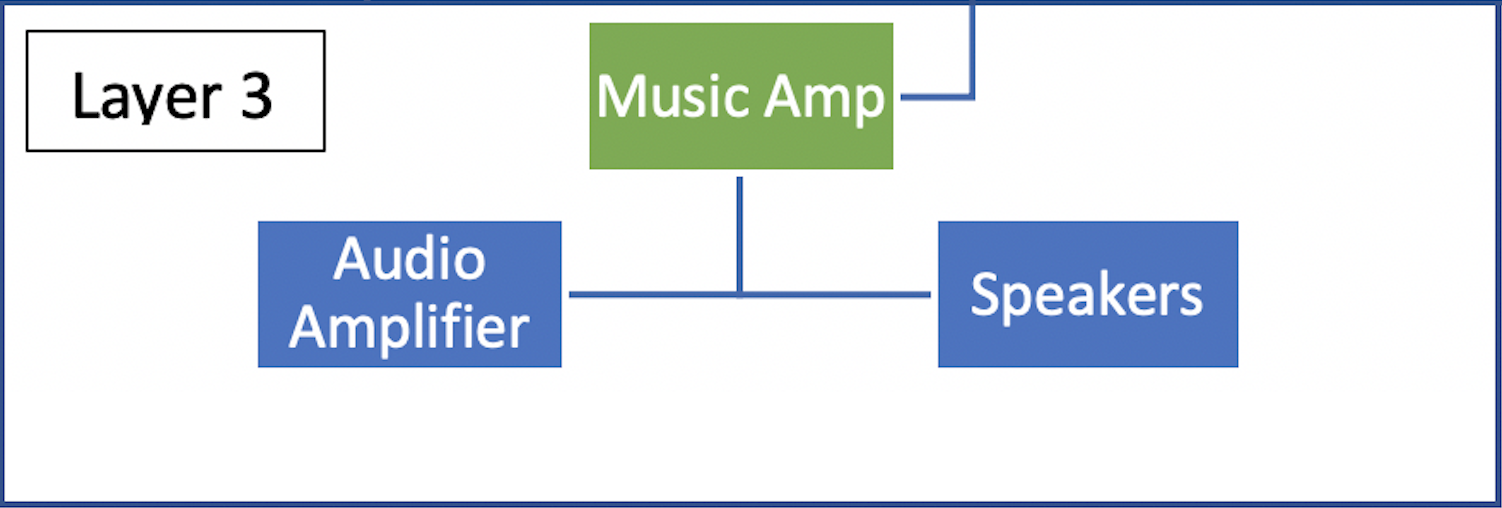
\includegraphics[width=0.60\textwidth]{images/subsystem3}
 \caption{Audio amplifier subsystem - speakers}
\end{figure}

\subsubsection{Assumptions}
It is assumed that there will be speakers available that will fit our specifications and that will be able to comfortably and safely fit in the backpack. We also assume that there are speakers powerful enough to emit vibrations that can be felt through the backpack we will use.

\subsubsection{Responsibilities}
The speakers have few responsibilities, in terms of custom functionality. They are simply meant to be the medium through which the user will feel the music/vibrations.

\subsubsection{Speakers Interfaces}

\begin {table}[H]
\caption {Speaker interfaces} 
\begin{center}
    \begin{tabular}{ | p{1cm} | p{6cm} | p{3cm} | p{3cm} |}
    \hline
    ID & Description & Inputs & Outputs \\ \hline
    \#1 & Connection to audio amplifier & \pbox{3cm}{ Audio amplification settings } & \pbox{3cm}{ Change in audio/vibration characteristics in backpack }  \\ \hline
    \#2 & Connection to music amplifier & \pbox{3cm}{ NA } & \pbox{3cm}{ Speakers receive amplified audio/music signals ready for output }  \\ \hline
    \end{tabular}
\end{center}
\end{table}

